\documentclass[10pt,twocolumn]{article}

% DaemonONE reusable research-paper template.
% Standard article class with two columns; no publisher-specific style is assumed.
\usepackage[a4paper,margin=0.72in,columnsep=0.25in]{geometry}
\usepackage[T1]{fontenc}
\usepackage{lmodern}
\usepackage{microtype}
\usepackage{graphicx}
\usepackage{booktabs}
\usepackage{tabularx}
\usepackage{array}
\usepackage{url}
\usepackage[hidelinks]{hyperref}
\raggedbottom
\usepackage[nameinlink,noabbrev]{cleveref}

\setlength{\columnseprule}{0pt}
\renewcommand{\thesection}{\Roman{section}}
\renewcommand{\thesubsection}{\thesection.\arabic{subsection}}
\renewcommand{\thesubsubsection}{\thesubsection.\arabic{subsubsection}}
\makeatletter
\renewcommand\subsection{\@startsection{subsection}{2}{\z@}{-3.25ex\@plus -1ex \@minus -.2ex}{1.5ex \@plus .2ex}{\normalfont\large\bfseries\raggedright}}
\renewcommand\subsubsection{\@startsection{subsubsection}{3}{\z@}{-3.25ex\@plus -1ex \@minus -.2ex}{1.5ex \@plus .2ex}{\normalfont\normalsize\bfseries\raggedright}}
\makeatother
\newcommand{\paperentry}[1]{\subsection{#1}}
\newcommand{\resourceRegistryName}{five-layer logical resource registry}
\newcommand{\doi}[1]{\url{https://doi.org/#1}}
\emergencystretch=1em

\title{Towards a Unified Local-First Computing Environment for Multi-Device Development}
\author{%
	\begin{minipage}{0.92\textwidth}
		\centering
		Dr.\ Swati R. Khokle\textsuperscript{1}, Bhavik D. Pawar\textsuperscript{2}, Shivam B. More\textsuperscript{2},\\ Tasbiya H. Shaikh\textsuperscript{2},
		Ishika S. Sharma\textsuperscript{2}\\[0.6em]
		\small
		\textsuperscript{1}Assistant Professor, Department of Computer Engineering,
		Guru Gobind Singh College of Engineering and Research Centre, Nashik, India\\[0.3em]
		\textsuperscript{2}Student, Department of Computer Engineering,
		Guru Gobind Singh College of Engineering and Research Centre, Nashik, India
	\end{minipage}
}
\date{01 November 2026}

\begin{document}

% The title and author span the page; the abstract stays in the left column.
\twocolumn[\maketitle]
\begin{abstract}
  Today's software development increasingly spans multiple personal devices, yet these environments often remain isolated, without cross-device visibility or consolidated resource awareness. Traditional cloud-centric paradigms move application state and execution to remote data centers, adding network latency, requiring persistent internet connectivity, and limiting user ownership and control. Service discovery and task coordination often rely on central servers, creating a single point of failure and limiting operation during network disconnection. 
  
  Existing research addresses local-first computing, device and service discovery, multi-device interaction, distributed resource management, distributed task execution, and metadata and resource discovery. However, these capabilities are generally studied separately and in different deployment contexts. Local-first research often does not extend to system-level resources such as containers, databases, active services, and Git repositories, while distributed resource management and FaaS edge frameworks generally target enterprise environments. Existing solutions therefore leave a gap for a unified, offline-aware, local-first layer that integrates metadata, services, resources, and task execution. 
  
  This paper presents DaemonONE, a proposed local-first distributed computing environment that provides a unified logical view across an individual's personal devices. The review establishes an architectural and conceptual foundation for investigating this integrated personal computing environment.
  \par\smallskip
  \noindent\textbf{Keywords---} \textit{\textbf{Local-first computing, multi-device systems, resource discovery, metadata management, peer-to-peer computing, distributed computing, controlled task execution.}}
\end{abstract}

\section{Introduction}\label{sec:introduction}
Software developer is now increasingly working with different personal devices such as laptops, desktops, home servers, and laboratory servers to perform tasks like testing, database hosting, compilation, and service management. Different devices are independent of each other, thus causing the distribution of repositories, databases, containers, and computing resources across different devices. The cloud-based approach has the issue of network latency and requirement for an uninterrupted internet connection, with less control and ownership of the data~\cite{ref2,ref21}. The disconnection of the network can cause further issues in the discovery and management of the devices~\cite{ref6,ref7}.

Local-first computing revolves around the concepts of data ownership, data locality, and limited reliance on central authorities~\cite{ref2,ref3}. Other work that has been done in the past includes decentralized device/service discovery~\cite{ref6,ref7}, multi-device interaction~\cite{ref17,ref18}, and distributed/edge resource management~\cite{ref14,ref15,ref23}. Yet again, these aspects have not been explored together but separately, providing an opportunity to bring them all together into one environment.

In this paper we present \textbf{DaemonONE}, a distributed computational system which gives a single view about the collection of the user’s devices. The system incorporates decentralized discovery of devices, indexing of device metadata, offline-aware resource management, service monitoring, searching across devices and controlled execution of predefined tasks for developers.

The rest of the paper is structured as follows. \Cref{sec:literature} provides the literature review, which gives a summary of the selected research papers. \Cref{sec:methodology} describes the research gap, proposed system, methodology, and architecture of DaemonONE. \Cref{sec:findings} analyzes the findings and compares the proposed system with existing distributed computing architectures. \Cref{sec:conclusion} concludes the paper and highlights future work.


\section{Literature Survey}\label{sec:literature}
Designing computing platforms for personal multi-device software development draws on several areas of parallel and distributed systems. The following subsections review six themes: local-first software and data consistency, device and service discovery, multi-device interaction and workflow migration, distributed resource management, distributed task execution, and metadata indexing. A comparative synthesis closes the survey and identifies the research gaps that motivate DaemonONE.

\paperentry{Data Overlay Mesh in Distributed Clouds Enabling Collaborative Applications (2025)}M. Simić et al.~\cite{ref1} present a logical overlay mesh that connects distributed cloud resources to enable collaborative applications. This technique offers a common abstraction for accessing distributed computing resources.

\paperentry{Local-First Software: You Own Your Data, in Spite of the Cloud (2019)}M. Kleppmann et al.~\cite{ref2} describe local-first software, emphasizing data ownership, locality, collaboration, and independence from central cloud services. They analyze design principles for responsive applications that preserve user control over data.
\paperentry{LoRe: A Programming Model for Verifiably Safe Local-First Software (2023)}J. Haas et al.~\cite{ref3} present LoRe, a programming model that applies formal methods to specify and verify safety properties in local-first software.
\paperentry{Distributed Computing with the Cloud (2024)}Y. Afek et al.~\cite{ref4} analyze distributed computing models that integrate local communication with cloud storage and computing, focusing on coordination of computing and communication resources.
\paperentry{Optimization of Resource-Aware Parallel and Distributed Computing: A Review (2025)}P. Czarnul et al.~\cite{ref5} review optimization approaches for resource-aware parallel and distributed computing, including resource modeling, scheduling, workload balancing, and optimization.
\paperentry{Multicast DNS (2013)}S. Cheshire and M. Krochmal \cite{ref6} describe Multicast DNS (mDNS), a protocol for resolving device names on a local network without a DNS server. It provides zero-configuration name resolution using multicast communication.
\paperentry{DNS Service Discovery (2013)}S. Cheshire and M. Krochmal \cite{ref7} describe DNS-based Service Discovery, which uses DNS records to advertise service types and connection details.
\paperentry{A Distributed Tracing Pipeline for Improving Locality Awareness of Microservices Applications (2024)}C. Colarusso et al.~\cite{ref8} present a distributed tracing pipeline that analyzes communication in microservices applications. They use tracing data to identify service relationships and improve locality awareness during placement.
\paperentry{Conflict-Free Replicated Data Types: An Overview (2018)}N. Preguiça \cite{ref9} surveys conflict-free replicated data types (CRDTs), which allow replicas to converge after updates are exchanged under their defined assumptions.
\paperentry{WireGuard: Next Generation Kernel Network Tunnel (2017)}J. A. Donenfeld \cite{ref10} presents WireGuard, a protocol for secure network tunnels that uses cryptographic mechanisms to protect peer communication.
\paperentry{A Function-as-a-Service Middleware for Decentralized Collaborative Edge Computing (2026)}C. Gonçalves et al.~\cite{ref11} present Function-as-a-Service middleware for decentralized edge computing, enabling edge nodes to discover one another and collaborate on function execution.
\paperentry{Behavioural Types for Local-First Software (2023)}R. Kuhn et al.~\cite{ref12} study behavioral types for local-first software, using protocol-based coordination and event logs to describe communication among autonomous nodes.
\paperentry{Resource-Aware Deployment of Dynamic DNNs over Multi-Tiered Interconnected Systems (2024)}C. Singhal et al.~\cite{ref13} present a scheme for deploying dynamic deep neural networks across mobile, edge, and cloud environments by placing model components according to resource conditions.
\paperentry{Scheduling of Distributed Applications on the Computing Continuum: A Survey (2023)}N. Mehran et al.~\cite{ref14} survey scheduling strategies for distributed applications across the computing continuum, considering execution time, energy, and cost.
\paperentry{Comprehensive Survey on Resource Management for IoT Applications in Edge-Fog-Cloud Environments (2025)}N. E. H. Boubaker et al.~\cite{ref15} survey resource management for IoT applications in edge-fog-cloud environments, including resource allocation, task scheduling, computation offloading, and service migration.
\paperentry{Decentralised Global Service Discovery for the Internet of Things (2024)}R. Kurte et al.~\cite{ref16} present a decentralized service-discovery approach for IoT systems using distributed hash tables, cryptographic service identifiers, and digital signatures on metadata.
\paperentry{Supporting Flexible and Transparent User Interface Distribution Across Mobile Devices (2024)}S. Oh et al.~\cite{ref17} propose a mechanism for distributing interface components across mobile devices through graphics-state serialization and cross-device communication.
\paperentry{Opportunistic Nudges for Task Migration Between Personal Devices (2024)}N. Joshi et al.~\cite{ref18} examine how visual prompts and device interactions can facilitate cross-device task migration and context transfer.
\paperentry{Resource-Aware Federated Data Analytics in Edge-Enabled IoT Systems (2024)}H. Khamfroush \cite{ref19} studies resource-aware federated data analytics in edge-enabled IoT systems. Participating devices compute over local data and send model parameters instead of transferring all data to one location.
\paperentry{A Distributed Learned Hash Table (2025)}S. Wang et al.~\cite{ref20} propose a distributed learned hash table that uses learned models for data location and retrieval. The model supports search and range queries in distributed systems.
\paperentry{End-to-End Slices to Orchestrate Resources and Services in the Cloud-to-Edge Continuum (2023)}F. Tusa and S. Clayman \cite{ref21} present a method for orchestrating computing and network resources, as well as services, between the cloud and edge using end-to-end slices.
\paperentry{A Decentralized Approach for Resource Discovery Using Metadata Replication in Edge Networks (2022)}I. Murturi and S. Dustdar \cite{ref22} propose a decentralized framework for resource discovery using metadata replication in edge networks. This framework allows devices to share and store resource metadata independently of a centralized repository.
\paperentry{Distributed Resource Scheduling in Edge Computing: Problems, Solutions, and Opportunities (2022)}Y. Sahni et al.~\cite{ref23} review methods for distributed resource scheduling in edge computing, including computation, storage, networking, device heterogeneity, and resource variability.
\paperentry{BarMan: A Run-Time Management Framework in the Resource Continuum (2022)}M. Zanella et al.~\cite{ref24} present BarMan, a runtime management framework that assigns tasks across heterogeneous resources while accounting for changes in resource availability and system performance.
\paperentry{Resource Provisioning and Allocation in Function-as-a-Service Edge-Clouds (2022)}O. Ascigil et al.~\cite{ref25} examine resource provisioning and allocation for latency-critical FaaS workloads in edge-cloud settings, including centralized and decentralized allocation policies.

\section{Proposed Methodology}\label{sec:methodology}
\subsection{Research Gap}\label{subsec:research-gap}
\subsubsection{Cloud-Centric Orchestration and Local-First Offline Resilience}
The literature distinguishes cloud-centric distributed computing from local-first systems in their approaches to resource coordination, network connectivity, and offline operation. Work on distributed and edge-cloud computing studies resource management, scheduling, service orchestration, and load balancing across distributed infrastructure \cite{ref5}, \cite{ref14}, \cite{ref15}, \cite{ref21}, \cite{ref23}. These approaches generally coordinate infrastructure whose participating components communicate over a network.


Local-first computing emphasizes local data ownership, local computation, and continued operation without a persistent connection to a central cloud service \cite{ref2}, \cite{ref3}, \cite{ref12}. Discovery mechanisms such as mDNS and DNS-SD provide zero-configuration discovery on local networks \cite{ref6}, \cite{ref7}. Local-first approaches therefore support operation during intermittent connectivity, while cloud and edge research offers methods for resource coordination and management.

DaemonONE aims to combine local-first operation with a distributed network of personal devices. It is designed to retain local metadata and the last-known state of a peer when that peer goes offline, allowing users to view their computing environment without a central cloud service.

\subsubsection{Mismatch in Resource Awareness Scope and Abstraction Levels}
The reviewed literature addresses resource awareness at different scopes and abstraction levels. Local-first research focuses on application data, state replication, consistency, and coordination among application replicas \cite{ref2}, \cite{ref3}, \cite{ref9}, \cite{ref12}. It provides mechanisms for managing application state during disconnection but generally does not address system-level developer resources such as active database services, Git repositories, containerized applications, or host-level resource telemetry.

In contrast, research on distributed resource management, edge computing, FaaS, and infrastructure orchestration focuses on allocation and execution within larger, heterogeneous infrastructures \cite{ref11}, \cite{ref13}, \cite{ref14}, \cite{ref15}, \cite{ref21}, \cite{ref24}, \cite{ref25}. These studies address computing capacity, virtual infrastructure, workloads, and services in edge-cloud or multi-domain environments.

This creates an abstraction-level gap in the reviewed literature. Local-first systems support autonomy and offline operation, while distributed resource management systems provide methods for resource awareness and workload coordination. Their integration for personal computers remains underdeveloped. DaemonONE addresses this gap with a logical registry of application resources, development services, and host resource information.

\subsubsection{Execution Security Trade-Offs in Distributed Environments}
The reviewed literature shows a trade-off between execution flexibility and access control in distributed systems. Edge FaaS and distributed execution platforms provide tools for controlled workload execution \cite{ref11}, \cite{ref21}, \cite{ref24}, \cite{ref25}, but generally focus on functions, services, and managed workloads rather than developers' tasks.

In a personal multi-device setup, remote shell access offers flexibility but increases security risks. DaemonONE instead restricts remote execution to approved development tasks. Each target daemon checks the requested task against its local whitelist before starting a process. The initial task set is \texttt{cargo build}, \texttt{cargo test}, \texttt{git status}, \texttt{docker compose up}, and \texttt{docker compose down}; interactive shell access is outside the system's scope.


\subsection{Proposed System}\label{subsec:proposed-system}
DaemonONE is designed to address resource fragmentation, cloud dependency, and offline fragility in personal multi-device software development. Unlike enterprise cluster managers and cloud orchestrators, it offers a local-first peer-to-peer environment for one software developer's personal devices.

The following subsections describe the DaemonONE architecture, discovery protocols, metadata indexing, offline-aware operation, resource monitoring, and controlled task execution.

\subsubsection{System Architecture}\label{subsec:architecture}
DaemonONE works on a decentralized, peer-to-peer, and local-first model, meaning that data processing and storage are done locally without depending on the centralized cloud servers. Devices share their resource metadata so that a complete overview of the computing environment is created while keeping local control.

A lightweight daemon named \texttt{daemononed} runs on each device to track its resources. Laptops, desktops, home servers, and lab nodes retain their own operating systems, hardware, storage, and services. DaemonONE tracks resources but does not physically consolidate CPU cores, memory, or storage. The architecture is shown in \Cref{fig:system-architecture}.
\begin{figure*}[!t]
	\centering
	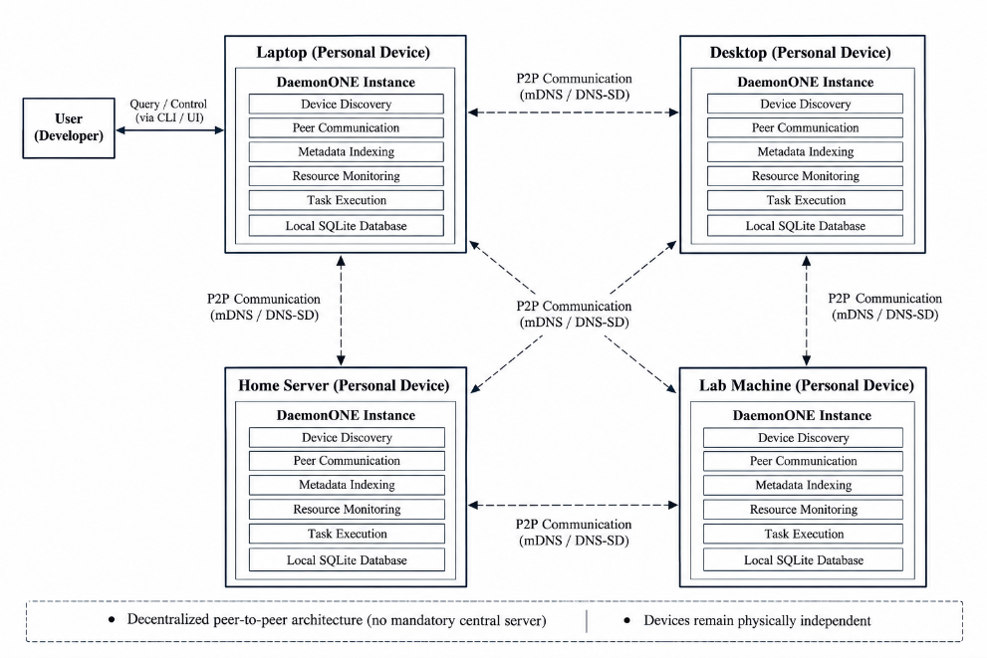
\includegraphics[width=0.94\textwidth]{images/system-architecture.png}
\caption{DaemonONE's local-first, peer-to-peer architecture across personal devices and their local daemons.}
	\label{fig:system-architecture}
\end{figure*}
\subsubsection{Device Discovery and Peer Communication}\label{subsec:discovery}
DaemonONE uses zero-configuration discovery and peer authentication to connect devices on a local network without manual infrastructure configuration.

\begin{enumerate}
  \item \textbf{Zero-configuration link discovery:} At start-up, each DaemonONE instance discovers participating devices and their advertised services on the local network using Multicast DNS (mDNS) \cite{ref6} and DNS-based Service Discovery (DNS-SD) \cite{ref7}. Both protocols support device or service discovery without a DNS server or manual configuration \cite{ref6}, \cite{ref7}.
  \item \textbf{Peer authentication:} Connections are limited to devices approved by the user. Each DaemonONE instance authenticates its authorized peers. The secure transport mechanism remains to be specified; WireGuard provides one relevant encrypted-tunnel approach \cite{ref10}.
  \item \textbf{Structured payload exchange:} After establishing a secure connection, each instance exchanges structured payloads containing node identity, local resource status, active-service information, and permitted tasks.
\end{enumerate}

\subsubsection{Metadata Indexing and Unified Resource Registry}\label{subsec:registry}
Instead of physically moving data, DaemonONE maintains a \resourceRegistryName{}. Each local daemon inspects the file system, active operating-system processes, container interfaces, and project folders on its device, then stores metadata in an embedded local database. The registry structure is summarized in \Cref{tab:resource-registry}.

\begin{table*}[!t]
	\centering
\caption{The five-layer logical resource registry records data, projects, services, host resources, and approved execution tasks for each device.}
	\label{tab:resource-registry}
	\begin{tabularx}{0.96\textwidth}{>{\raggedright\arraybackslash}p{0.17\textwidth} X X}
		\toprule
		\textbf{Layer} & \textbf{Description \& tracked entities} & \textbf{System scope \& function} \\
		\midrule
		1. Data Layer
		& File names, paths, folder metadata, file sizes, and modification timestamps
		& Identifies the physical host location of files; not a distributed filesystem \\
		2. Project Layer
		& Git repositories, active branches, environment files (\texttt{.env}), and build targets
		& Maps software project locations and active source-code repositories \\
		3. Service Layer
		& PostgreSQL, MySQL, Redis, Docker containers, local API servers, and web ports
		& Indexes active backend services and accessible development ports \\
		4. Resource Layer
		& CPU utilization, RAM usage, available disk capacity, and network latency
		& Provides hardware telemetry; task-placement policies remain future work \\
		5. Execution Layer
		& Whitelisted tasks such as \texttt{cargo build}, \texttt{cargo test}, \texttt{git status}, \texttt{docker compose up}, and \texttt{docker compose down}
		& Authorizes and routes pre-approved development tasks \\
		\bottomrule
	\end{tabularx}
\end{table*}

The \resourceRegistryName{} provides a unified view of the developer's heterogeneous devices and identifies the device that physically stores each asset.
\subsubsection{Offline-Aware Metadata Management}\label{subsec:metadata}
Operational continuity during network disconnection is a core local-first principle \cite{ref2}. DaemonONE's offline-aware behavior is designed to support the following:
\begin{enumerate}
  \item \textbf{Last-known state persistence:} When a device is unreachable because of a network or power failure, other active daemons retain its last-known metadata, services, and resource state in their local indexes.
  \item \textbf{Reconnection synchronization:} When a disconnected device reconnects, participating daemons exchange updated local index data. The conflict-resolution policy for concurrent changes remains to be specified and evaluated.
  \item \textbf{Local-first operation:} Users can query the logical registry and view previously stored details for resources associated with disconnected devices, consistent with local-first principles \cite{ref2}.
\end{enumerate}

\subsubsection{Resource and Service Monitoring}\label{subsec:monitoring}
DaemonONE is designed to monitor host hardware resources and development services in near real time. The monitoring involves three activities:

\begin{itemize}
  \item \textbf{System-resource telemetry:} Local daemons monitor CPU and RAM usage, available disk space, network connectivity, and node availability. Related work on locality-aware tracing informs analysis of service relationships \cite{ref8}.
  \item \textbf{Service and process monitoring:} Using operating-system process data and container interfaces such as the Docker API, DaemonONE is designed to detect and register active services, including PostgreSQL, MySQL, Redis, containerized services, and local web servers.
  \item \textbf{Logical abstraction:} Hardware metrics and service information are represented in the consolidated resource registry for developer visibility. Hardware resources are not physically combined or dynamically pooled across participating nodes.
\end{itemize}

\subsubsection{Cross-Device Search and Controlled Task Execution}\label{subsec:execution}
\paragraph{Cross-device search.} Developers can use a command-line or desktop interface to find project repositories, files, environment settings, running containers, or hardware capabilities across connected devices. Results identify the device that contains each resource. The registry supporting these queries is summarized in \Cref{tab:resource-registry}.

\paragraph{Controlled task execution.} DaemonONE is designed to launch approved build or test processes on another personal device, such as running a resource-intensive build on a desktop while working from a laptop. The initial task set is \texttt{cargo build}, \texttt{cargo test}, \texttt{git status}, \texttt{docker compose up}, and \texttt{docker compose down}.
\begin{itemize}
  \item \textbf{Pre-execution validation:} The target daemon checks each requested task against its local authorization whitelist before starting a child process.
  \item \textbf{Output streaming:} The target daemon captures standard output, standard error, and the process exit code, then returns them to the requesting device.
  \item \textbf{Scope boundary:} Arbitrary remote shell execution, including interactive SSH or shell sessions, is outside the system's scope.
\end{itemize}


\section{Findings}\label{sec:findings}
The literature review and the DaemonONE design highlight how distributed computing systems address resource discovery, state consistency, execution safety, and offline resilience. The comparison in \Cref{tab:architecture-comparison} summarizes these findings across the approaches surveyed. Related work also provides precedents in overlay resource access \cite{ref1}, locality-aware tracing \cite{ref8}, resource-aware deployment \cite{ref13}, and federated analytics \cite{ref19}.
\begin{table*}[!t]
	\centering
\caption{Comparison of centralized cloud, edge FaaS, local-first, peer-to-peer discovery, and DaemonONE approaches across network topology, cloud dependence, offline operation, resource scope, execution, and deployment context.}
	\label{tab:architecture-comparison}
	\small
	\begin{tabularx}{0.98\textwidth}{>{\raggedright\arraybackslash}p{0.14\textwidth}*{5}{>{\raggedright\arraybackslash}X}}
		\toprule
		\textbf{Dimension}
		& \textbf{Centralized Cloud and Cloud Slicing \cite{ref4}, \cite{ref21}}
		& \textbf{Edge FaaS and Distributed Middleware \cite{ref11}, \cite{ref25}}
		& \textbf{Local-First Software \cite{ref2}, \cite{ref3}, \cite{ref9}}
		& \textbf{P2P Discovery \& Resource Lookup \cite{ref16}, \cite{ref20}, \cite{ref22}}
		& \textbf{Proposed DaemonONE} \\
		\midrule
		Network topology
		& Cloud/edge infrastructure with centralized or multi-domain coordination \cite{ref4}, \cite{ref21}
		& Distributed edge/cloud execution \cite{ref11}, \cite{ref25}
		& Local replicas with peer synchronization \cite{ref2}, \cite{ref3}, \cite{ref9}
		& Decentralized P2P overlays and clusters \cite{ref16}, \cite{ref22}
		& Decentralized personal-device P2P \\
		\addlinespace
		Cloud dependency
		& Cloud/edge infrastructure is part of the deployment model \cite{ref4}, \cite{ref21}
		& Edge-cloud infrastructure \cite{ref11}, \cite{ref25}
		& Emphasizes local operation and reduced dependence on centralized services \cite{ref2}
		& Decentralized discovery and lookup \cite{ref16}, \cite{ref22}
		& No mandatory central cloud server \\
		\addlinespace
		Offline operation
		& Depends on participating infrastructure and network connectivity \cite{ref4}, \cite{ref21}
		& Depends on participating edge/cloud resources and connectivity \cite{ref11}, \cite{ref25}
		& Strong emphasis on local operation during disconnection \cite{ref2}, \cite{ref3}, \cite{ref9}
		& Provides decentralized lookup when the peer overlay is reachable; offline behavior is not specified \cite{ref16}, \cite{ref20}, \cite{ref22}
		& Retains last-known metadata and device status \\
		\addlinespace
		Resource scope
		& Compute, network, infrastructure, and service resources \cite{ref4}, \cite{ref21}
		& Functions, workloads, and edge-cloud resources \cite{ref11}, \cite{ref25}
		& Application data and replicated state \cite{ref2}, \cite{ref3}, \cite{ref9}
		& Services, resources, metadata, and distributed lookup \cite{ref16}, \cite{ref20}, \cite{ref22}
		& Five-layer logical registry covering data, projects, services, resources, and execution \\
		\addlinespace
		Execution model
		& Distributed workload/resource orchestration \cite{ref4}, \cite{ref21}
		& Function- and service-oriented execution \cite{ref11}, \cite{ref25}
		& Primarily application-level local execution and synchronization \cite{ref2}, \cite{ref3}
		& Primarily discovery and resource lookup \cite{ref16}, \cite{ref20}, \cite{ref22}
		& Controlled execution of predefined development tasks \\
		\addlinespace
		Deployment context
		& Cloud-to-edge and distributed infrastructure \cite{ref4}, \cite{ref21}
		& Edge-cloud and distributed service environments \cite{ref11}, \cite{ref25}
		& Local-first collaborative applications \cite{ref2}, \cite{ref3}, \cite{ref9}
		& IoT, edge, and decentralized resource environments \cite{ref16}, \cite{ref20}, \cite{ref22}
		& Personal multi-device developer environment \\
		\bottomrule
	\end{tabularx}
\end{table*}
\paragraph{Summary of Findings and System Design Implications.}\label{subsec:implications}
The reviewed domains offer components relevant to DaemonONE, including zero-configuration device and service discovery \cite{ref6}, \cite{ref7}, local-first computing \cite{ref2}, \cite{ref3}, \cite{ref9}, decentralized resource discovery \cite{ref16}, \cite{ref22}, distributed resource management \cite{ref5}, \cite{ref14}, \cite{ref15}, \cite{ref23}, and controlled distributed execution \cite{ref11}, \cite{ref24}, \cite{ref25}. These features are generally studied in other applications or deployment contexts. DaemonONE combines a local-first peer-to-peer approach, a \resourceRegistryName{} for data, projects, services, system resources, and controlled execution, and an authorization model for remote development tasks. It integrates capabilities from the reviewed literature and is not a substitute for the individual systems surveyed.

\section{Conclusion}\label{sec:conclusion}
Personal computing environments increasingly include laptops, desktop computers, and home or laboratory servers. Projects, repositories, development services, and system resources may still be managed separately on each device. This creates an opportunity to combine local-first computing, decentralized device and service discovery, metadata management, inter-device communication, and distributed resource management in one personal computing environment. This paper proposed \textbf{DaemonONE}, a local-first distributed computing platform that provides a unified logical view of personal devices through lightweight background daemons, decentralized device discovery, offline-aware metadata handling, and a \resourceRegistryName{} covering data, projects, services, resources, and execution.

The proposed architecture provides a basis for coordinating development resources across personal devices, but it has not yet been empirically evaluated for performance, usability, or efficiency. Future work will implement DaemonONE across diverse devices and measure resource-discovery and metadata-synchronization overhead, task-execution latency, monitoring accuracy, and usability. Further work may address stronger execution security policies, conflict resolution during disconnection and reconnection synchronization, discovery of relationships between development services, and resource-aware task scheduling.


\clearpage 
\begin{thebibliography}{25}
\bibitem{ref1} M. Simi\'{c}, J. Dedei\'{c}, M. Stojkov, and I. Proki\'{c}, ``Data overlay mesh in distributed clouds allowing collaborative applications,'' \emph{IEEE Access}, vol. 13, pp. 6180--6203, 2025, \doi{10.1109/ACCESS.2024.3525336}.
\bibitem{ref2} M. Kleppmann, A. Wiggins, P. van Hardenberg, and M. McGranaghan, ``Local-first software: You own your data, in spite of the cloud,'' in \emph{Proc. ACM SIGPLAN Int. Symp. New Ideas, New Paradigms, and Reflections on Programming and Software (Onward! '19)}, 2019, pp. 154--178, \doi{10.1145/3359591.3359737}.
	
\bibitem{ref3} J. Haas, R. Mogk, E. Yanakieva, A. Bieniusa, and M. Mezini, ``LoRe: A programming model for verifiably safe local-first software,'' in \emph{Proc. 37th European Conf. Object-Oriented Programming (ECOOP 2023)}, LIPIcs, vol. 263, 2023, pp. 12:1--12:15, \doi{10.4230/LIPIcs.ECOOP.2023.12}.
	
\bibitem{ref4} Y. Afek, G. Giladi, and B. Patt-Shamir, ``Distributed computing with the cloud,'' \emph{Distributed Computing}, vol. 37, pp. 1--18, 2024, \doi{10.1007/s00446-024-00460-w}.
	
\bibitem{ref5} P. Czarnul et al., ``Optimization of resource-aware parallel and distributed computing: A review,'' \emph{The Journal of Supercomputing}, vol. 81, no. 7, Art. no. 848, 2025, \doi{10.1007/s11227-025-07295-7}.
	
\bibitem{ref6} S. Cheshire and M. Krochmal, ``Multicast DNS,'' RFC 6762, Internet Engineering Task Force, Feb. 2013, \doi{10.17487/RFC6762}.
	
\bibitem{ref7} S. Cheshire and M. Krochmal, ``DNS-based service discovery,'' RFC 6763, Internet Engineering Task Force, Feb. 2013, \doi{10.17487/RFC6763}.
	
\bibitem{ref8} C. Colarusso, A. De Caro, I. Falco, L. Goglia, and E. Zimeo, ``A distributed tracing pipeline for improving locality awareness of microservices applications,'' \emph{Software: Practice and Experience}, vol. 54, no. 6, pp. 1118--1140, 2024, \doi{10.1002/spe.3317}.
	
	\bibitem{ref9} N. Pregui\c{c}a, ``Conflict-free replicated data types: An overview,'' arXiv:1806.10254, 2018.
	
\bibitem{ref10} J. A. Donenfeld, ``WireGuard: Next generation kernel network tunnel,'' in \emph{Proc. Network and Distributed System Security Symp. (NDSS)}, San Diego, CA, USA, 2017, pp. 1--12, \doi{10.14722/ndss.2017.23160}.
	
\bibitem{ref11} C. Gon\c{c}alves, J. Sim\~{a}o, and L. Veiga, ``A function-as-a-service middleware for decentralized collaborative edge computing,'' \emph{Future Generation Computer Systems}, vol. 175, Art. no. 108069, 2026, \doi{10.1016/j.future.2025.108069}.
	
\bibitem{ref12} R. Kuhn, H. C. Melgratti, and E. Tuosto, ``Behavioural types for local-first software,'' in \emph{Proc. 37th European Conf. Object-Oriented Programming (ECOOP 2023)}, LIPIcs, vol. 263, 2023, pp. 15:1--15:28, \doi{10.4230/LIPIcs.ECOOP.2023.15}.
	
\bibitem{ref13} C. Singhal, Y. Wu, F. Malandrino, M. Levorato, and C. F. Chiasserini, ``Resource-aware deployment of dynamic DNNs over multi-tiered interconnected systems,'' in \emph{Proc. IEEE INFOCOM 2024}, Vancouver, BC, Canada, 2024, \doi{10.1109/INFOCOM52122.2024.10621218}.
	
\bibitem{ref14} N. Mehran, D. Kimovski, H. Hellwagner, D. Roman, A. Soylu, and R. Prodan, ``Scheduling of distributed applications on the computing continuum: A survey,'' in \emph{Proc. IEEE/ACM 16th Int. Conf. Utility and Cloud Computing (UCC 2023)}, 2023, pp. 1--6, \doi{10.1145/3603166.3632540}.
	
\bibitem{ref15} N. El Houda Boubaker, K. Zarour, N. Guermouche, and D. Benmerzoug, ``A comprehensive survey on resource management for IoT applications in edge-fog-cloud environments,'' \emph{IEEE Access}, vol. 13, pp. 111892--111925, 2025, \doi{10.1109/ACCESS.2025.3583584}.
	
\bibitem{ref16} R. Kurte, Z. Salcic, and K. I.-K. Wang, ``Decentralised global service discovery for the Internet of Things,'' \emph{Sensors}, vol. 24, no. 7, Art. no. 2196, 2024, \doi{10.3390/s24072196}.
	
\bibitem{ref17} S. Oh, A. Kim, S. Lee, K. Lee, D. R. Jeong, S. Y. Ko, and I. Shin, ``Supporting flexible and transparent user interface distribution across mobile devices,'' \emph{IEEE Transactions on Mobile Computing}, vol. 23, no. 8, pp. 8398--8417, 2024, \doi{10.1109/TMC.2024.3349561}.
	
\bibitem{ref18} N. Joshi et al., ``Opportunistic nudges for task migration between personal devices,'' in \emph{Extended Abstracts of the 2024 CHI Conference on Human Factors in Computing Systems (CHI EA '24)}, Honolulu, HI, USA, 2024, Art. no. 256, pp. 1--8, \doi{10.1145/3613905.3651037}.
	
\bibitem{ref19} H. Khamfroush, ``Resource-aware federated data analytics in edge-enabled IoT systems,'' \emph{Proceedings of the AAAI Symposium Series}, vol. 3, no. 1, p. 305, 2024, \doi{10.1609/aaaiss.v3i1.31219}.
	
\bibitem{ref20} S. Wang, Y. Liu, X. Zhang, L. Hu, and C. Qian, ``A distributed learned hash table,'' in \emph{Proc. IEEE 33rd Int. Conf. on Network Protocols (ICNP)}, Seoul, South Korea, 2025, pp. 1--11, \doi{10.1109/ICNP65844.2025.11192384}.
	
\bibitem{ref21} F. Tusa and S. Clayman, ``End-to-end slices to orchestrate resources and services in the cloud-to-edge continuum,'' \emph{Future Generation Computer Systems}, vol. 141, pp. 473--488, 2023, \doi{10.1016/j.future.2022.11.026}.
	
\bibitem{ref22} I. Murturi and S. Dustdar, ``A decentralized approach for resource discovery using metadata replication in edge networks,'' \emph{IEEE Transactions on Services Computing}, vol. 15, no. 5, pp. 2526--2537, 2022, \doi{10.1109/TSC.2021.3082305}.
	
\bibitem{ref23} Y. Sahni, J. Cao, L. Yang, and S. Wang, ``Distributed resource scheduling in edge computing: Problems, solutions, and opportunities,'' \emph{Computer Networks}, vol. 219, Art. no. 109430, 2022, \doi{10.1016/j.comnet.2022.109430}.
	
\bibitem{ref24} M. Zanella, F. Sciamanna, and W. Fornaciari, ``BarMan: A run-time management framework in the resource continuum,'' \emph{Sustainable Computing: Informatics and Systems}, vol. 35, Art. no. 100663, 2022, \doi{10.1016/j.suscom.2022.100663}.
	
\bibitem{ref25} O. Ascigil, A. G. Tasiopoulos, T. K. Phan, V. Sourlas, I. Psaras, and G. Pavlou, ``Resource provisioning and allocation in function-as-a-service edge-clouds,'' \emph{IEEE Transactions on Services Computing}, vol. 15, no. 4, pp. 2410--2424, 2022, \doi{10.1109/TSC.2021.3052139}.
	
\end{thebibliography}

\end{document}
